\pdfminorversion=4

% Modos:
% Definir el comando \handoutmode como "1" para compilar las diapositivas en
% modo handout
% al pdf generado ejecutarle el siguiente comando para poner varias diapo en una misma pagina:
%    pdfnup FILE.pdf --nup 2x3 --no-landscape --paper letterpaper --frame True
%
% Definir \handoutmode como algo distinto de "1" para compilar las diapositivas
% normalmente.
%
% Para configurar el modo desde afuera (la linea de comandos de latex) correr
% la compilacion como:
%
%   latex -output-directory=tmp -output-format=pdf '\def\handoutmode{1}\include{FILE.tex}'
%
\if\handoutmode1
    \documentclass[professionalfonts,handout]{beamer}
    \setbeameroption{show notes}
    \setbeamertemplate{note page}{\insertnote}
    \setbeamercolor{background canvas}{bg=white}
\else
    \documentclass[professionalfonts]{beamer}
\fi


% Template original the Beamer: Copyright 2004 by Till Tantau <tantau@users.sourceforge.net>.


\mode<presentation>
{
  \usetheme{metropolis}
  % or ...

  %\setbeamercovered{transparent} %hace que lo que esta covered se muestre transparente
}

\setbeamertemplate{navigation symbols}{}%remove navigation symbols

\usepackage[english]{babel}

\usepackage[latin1]{inputenc}

\usepackage{times}
\usepackage[T1]{fontenc}

% para poder escribir codigo fuente en las diapositivas
\usepackage{listings}

% para graficar diagramas simples y arboles de jerarquias
\usepackage{tikz}
\usepackage{tikz-qtree}
\usetikzlibrary{matrix,positioning}
\usetikzlibrary{shapes,arrows,chains,calc,decorations.pathmorphing}

\usepackage{xcolor}
\definecolor{darkgreen}{rgb}{0,.5,0}
\definecolor{darkblue}{rgb}{0,0,.7}
\lstdefinestyle{normal}{language=C++,       % lenguaje C++
   numbers=left,                            % enumerar las lineas
   keywordstyle=\color{darkblue}\textbf,    % color de las keywords
   stringstyle=\color{red},                 % color de los strings
   commentstyle=\color{darkgreen},          % color de los comentarios
   basicstyle=\color{black}\ttfamily\footnotesize\bfseries,     % color del texto en general
   morecomment=[l][\color{magenta}]{\#},    % coloreamos las intrucciones del precompilador (todo lo que empieza con #)
   ndkeywords={NULL,nullptr,siz,zer,mov,add},               % definimos una nuevas keywords como NULL y nullptr
   ndkeywordstyle=\color{violet},           % y las nuevas keywords tendran este color
   frame=simple,                            % simple, sin ningun marco o frame alrededor del codigo
   basewidth={0.55em,0.55em}                % tamano de las letras/lineas. usado para reducir el whitespace entre estas
}

\lstdefinestyle{normal33}{language=C++,       % lenguaje C++
   numbers=left,                            % enumerar las lineas
   keywordstyle=\color{darkblue}\textbf,    % color de las keywords
   stringstyle=\color{red},                 % color de los strings
   commentstyle=\color{darkgreen},          % color de los comentarios
   basicstyle=\color{black}\ttfamily\footnotesize\bfseries,     % color del texto en general
   morecomment=[l][\color{magenta}]{\#},    % coloreamos las intrucciones del precompilador (todo lo que empieza con #)
   ndkeywords={NULL,nullptr},               % definimos una nuevas keywords como NULL y nullptr
   ndkeywordstyle=\color{violet},           % y las nuevas keywords tendran este color
   frame=simple,                            % simple, sin ningun marco o frame alrededor del codigo
   basewidth={0.55em,0.55em}                % tamano de las letras/lineas. usado para reducir el whitespace entre estas
}
%mismo estilo, sin numeros
\lstdefinestyle{normalnonumbers}{language=C++,
   keywordstyle=\color{darkblue}\textbf,
   stringstyle=\color{red},           
   commentstyle=\color{darkgreen},    
   basicstyle=\color{black}\ttfamily\footnotesize\bfseries,
   morecomment=[l][\color{magenta}]{\#},
   ndkeywords={NULL,nullptr,move,add},          
   ndkeywordstyle=\color{violet}, 
   frame=simple,
   basewidth={0.55em,0.55em}
}


% mismo estilo pero todos los colores estan mas debiles como si se volvieran transparentes
% usado para poder resaltar el codigo.
\lstdefinestyle{dimmided}{language=C++,
   keywordstyle=\color{darkblue!30}\textbf,
   stringstyle=\color{red!30},
   commentstyle=\color{darkgreen!30},
   basicstyle=\color{black!30}\ttfamily\footnotesize\bfseries,
   morecomment=[l][\color{magenta!30}]{\#},
   ndkeywords={NULL,nullptr,siz,zer,mov,add},
   ndkeywordstyle=\color{violet!30}, 
   moredelim=**[is][\only<+->{\color{black}\lstset{style=normal}}]{@}{@}, % definimos que las lineas entre arrobas (@) tendran el estilo normal (con los colores a toda intensidad)
   frame=simple,
   basewidth={0.55em,0.55em}
}
\lstdefinestyle{dimmided42}{language=C++,
   keywordstyle=\color{darkblue!30}\textbf,
   stringstyle=\color{red!30},
   commentstyle=\color{darkgreen!30},
   basicstyle=\color{black!30}\ttfamily\footnotesize\bfseries,
   morecomment=[l][\color{magenta!30}]{\#},
   ndkeywords={NULL,nullptr,siz,zer,mov,add},
   ndkeywordstyle=\color{violet!30}, 
   moredelim=**[is][{\color{black}\lstset{style=normal}}]{@}{@}, % definimos que las lineas entre arrobas (@) tendran el estilo normal (con los colores a toda intensidad)
   frame=simple,
   basewidth={0.55em,0.55em}
}

\lstdefinelanguage{json}{
    literate=
     *{:}{{{\color{violet}{:}}}}{1}
      {,}{{{\color{violet}{,}}}}{1}
      {\{}{{{\color{darkgreen}{\{}}}}{1}
      {\}}{{{\color{darkgreen}{\}}}}}{1}
      {[}{{{\color{darkgreen}{[}}}}{1}
      {]}{{{\color{darkgreen}{]}}}}{1},
}


\lstdefinestyle{normaljson}{language=json,  % lenguaje json
   numbers=left,                            % enumerar las lineas
   keywordstyle=\color{darkblue}\textbf,    % color de las keywords
   stringstyle=\color{red},                 % color de los strings
   commentstyle=\color{red},                % color de los comentarios
   basicstyle=\color{black}\ttfamily\footnotesize\bfseries,     % color del texto en general
   morecomment=[l][\color{magenta}]{\#},    % coloreamos las intrucciones del precompilador (todo lo que empieza con #)
   ndkeywords={NULL,nullptr},               % definimos una nuevas keywords como NULL y nullptr
   ndkeywordstyle=\color{violet},           % y las nuevas keywords tendran este color
   frame=simple,                            % simple, sin ningun marco o frame alrededor del codigo
   basewidth={0.55em,0.55em}                % tamano de las letras/lineas. usado para reducir el whitespace entre estas
}

\lstdefinelanguage{http}{
    morekeywords={
        GET,
        PUT,
        POST,
        DELETE
    }
}

\lstdefinestyle{normalhttp}{language=http,  % lenguaje HTTP
   numbers=left,                            % enumerar las lineas
   keywordstyle=\color{darkblue}\textbf,    % color de las keywords
   stringstyle=\color{red},                 % color de los strings
   commentstyle=\color{red},                % color de los comentarios
   basicstyle=\color{black}\ttfamily\footnotesize\bfseries,     % color del texto en general
   morecomment=[l][\color{magenta}]{\#},    % coloreamos las intrucciones del precompilador (todo lo que empieza con #)
   ndkeywords={NULL,nullptr},               % definimos una nuevas keywords como NULL y nullptr
   ndkeywordstyle=\color{violet},           % y las nuevas keywords tendran este color
   frame=simple,                            % simple, sin ningun marco o frame alrededor del codigo
   basewidth={0.55em,0.55em}                % tamano de las letras/lineas. usado para reducir el whitespace entre estas
}

% Pone las constantes numericas con color (violeta en este caso):
% - los numeros que estan dentro de un string/comentarios NO son coloreados
% - los numeros por fuera que pertenecen a una palabra SON coloreados 
%   (buf1, por ejemplo, el "1" es coloreado cuando no lo deberias. UPS!!)
% - No incluye el signo
% 
%\lstset{literate=%
%  *{0}{{{\color{violet}0}}}1
%   {1}{{{\color{violet}1}}}1
%   {2}{{{\color{violet}2}}}1
%   {3}{{{\color{violet}3}}}1
%   {4}{{{\color{violet}4}}}1
%   {5}{{{\color{violet}5}}}1
%   {6}{{{\color{violet}6}}}1
%   {7}{{{\color{violet}7}}}1
%   {8}{{{\color{violet}8}}}1
%   {9}{{{\color{violet}9}}}1
%}

% Para resaltar lineas de codigo usando \btLstHLB{range} y \btLstHLB<overlay>{range}:
% Por ejemplo, 
%  \btLstHLB{3}       linea 3 resaltada
%  \btLstHLB{1-5}     lineas de la 1 a la 5 resaltadas
%  \btLstHLB<2>{3}    linea 3 resaltada solo en el slide 2
%
% \btLstHLB usa un color azul mientras que \btLstHLR usa un color rojo como fondo
\usepackage{lstlinebgrd}
\makeatletter
\newcount\bt@rangea
\newcount\bt@rangeb

\newcommand\btIfInRange[2]{%
   \global\let\bt@inrange\@secondoftwo%
   \edef\bt@rangelist{#2}%
   \foreach \range in \bt@rangelist {%
      \afterassignment\bt@getrangeb%
      \bt@rangea=0\range\relax%
      \pgfmathtruncatemacro\result{ ( #1 >= \bt@rangea) && (#1 <= \bt@rangeb) }%
      \ifnum\result=1\relax%
      \breakforeach%
      \global\let\bt@inrange\@firstoftwo%
      \fi%
   }%
   \bt@inrange%
}
\newcommand\bt@getrangeb{%
   \@ifnextchar\relax%
   {\bt@rangeb=\bt@rangea}%
   {\@getrangeb}%
}
\def\@getrangeb-#1\relax{%
   \ifx\relax#1\relax%
      \bt@rangeb=100000%   \maxdimen is too large for pgfmath
   \else%
      \bt@rangeb=#1\relax%
   \fi%
}

%%%%%%%%%%%%%%%%%%%%%%%%%%%%%%%%%%%%%%%%%%%%%%%%%%%%%%%%%%%%%%%%%%%%%%%%%%%%%%
%
% \btLstHL<overlay spec>{range list}
%
\newcommand<>{\btLstHLB}[1]{%
   \only#2{\btIfInRange{\value{lstnumber}}{#1}{\color{blue!30}}% blue
   {\def\lst@linebgrdcmd####1####2####3{}}}%
}%
\newcommand<>{\btLstHLR}[1]{%
   \only#2{\btIfInRange{\value{lstnumber}}{#1}{\color{red!30}}% red
   {\def\lst@linebgrdcmd####1####2####3{}}}%
}%
%
%
%%%%%%%%%%%%%%%%%%%%%%

\makeatother


% sin fecha
\date{}

\author[7542]{Di Paola Mart\'in \\ \texttt{martinp.dipaola <at> gmail.com} }

\institute[Universidad de Buenos Aires]
{
   Facultad de Ingenier\'ia\\
   Universidad de Buenos Aires
}

% Definimos una imagen para que este en cada slide
%\pgfdeclareimage[height=0.5cm]{university-logo}{imgs/fiuba.png}
%\logo{\pgfuseimage{university-logo}}

%% Definir estas en el documento final
%%
%% \title%
%% {Programaci\'on gen\'erica y templates en C++}
%%
%% \subject{Programaci\'on gen\'erica y templates en C++}


%%%%%
% At begin of each Section do nothing; at each Subsection show the Section and Subsection names
% If the Section doesn't have a Subsection, then YOU must to add a unnumbered Subsection like \subsection*{}
% so the AtBeginSubsection will get triggered
\AtBeginSection{}
\AtBeginSubsection[\frame{\subsectionpage}]{\frame{\subsectionpage}}
%
%%%%%




\title%
{Programaci\'on gen\'erica y templates en C++}

\subject{Programaci\'on gen\'erica y templates en C++}

\begin{document}

\begin{frame}
   \titlepage
\end{frame}

\begin{frame}{De qu\'e va esto?}
   \tableofcontents
\end{frame}


\section{Programaci\'on gen\'erica}
\subsection{Motivaci\'on}

\begin{frame}[fragile]{Juego de buscar diferencias}
   \begin{columns}
      \begin{column}{.5\linewidth}
         \begin{lstlisting}[style=normal,linebackgroundcolor={%
         \only<1>{\def\lst@linebgrdcmd####1####2####3{}}%
         \btLstHLB<2>{2}% espacio
         \btLstHLB<3>{6}% operador asignacion
         \btLstHLB<4>{10}% constructor por copia
   }]
class Array_int {
   int data[64];

   public:
   void set(int p, int v){
      data[p] = v;
   }

   int get(int p) {
      return data[p];
   }
};
         \end{lstlisting}
      \end{column}
      \begin{column}{.45\linewidth}
         \begin{lstlisting}[style=normal,linebackgroundcolor={%
         \only<1>{\def\lst@linebgrdcmd####1####2####3{}}%
         \btLstHLB<2>{2}% espacio
         \btLstHLB<3>{6}% operador asignacion
         \btLstHLB<4>{10}% constructor por copia
   }]
class Array_char {
   char data[64];

   public:
   void set(int p, char v){
      data[p] = v;
   }

   char get(int p) {
      return data[p];
   }
};
         \end{lstlisting}
      \end{column}
   \end{columns}
\only<2>{Reserva de espacio distintos}
\only<3>{Invocaci\'on de c\'odigo distintos: operador asignaci\'on}
\only<4>{Operador copia tambi\'en (y hay otros m\'as...)}
\end{frame}
\note[itemize] {
\item Imaginemos que necesitamos un array de \lstinline[style=normal]!64 int!s asi como tambi\'en de \lstinline[style=normal]!64 char!s. De las dos implementaciones, que diferencias hay?
\item Aunque no lo parezca, hay diferencias importantes desde el punto de vista del compilador y del c\'odigo m\'aquina generado.
\item Primero, reservan espacios distintos: \lstinline[style=normal]!64*sizeof(int)! contra \lstinline[style=normal]!64*sizeof(char)!
\item Segundo, invocan a c\'odigo (operadores) distintos: por ejemplo el operador asignaci\'on
\item Otros c\'odigos tambi\'en: el constructor por copia, posiblemente el constructor por default y el destructor.
\item Y todas estas diferencias por tan solo debido al cambio del tipo \lstinline[style=normal]!int! por \lstinline[style=normal]!char!
}


\begin{frame}[plain,fragile]{Alternariva I: void*}
   \begin{columns}[t]
      \begin{column}{.55\linewidth}
         \begin{lstlisting}[style=normal,linebackgroundcolor={%
               \only<1>{\def\lst@linebgrdcmd####1####2####3{}}%
               \btLstHLB<2>{7-8}% memcpy, copia bit a bit
               \btLstHLB<3>{12}% casteo!
         }]
class Array {
   void *data;    
   size_t sizeobj;

   public:
   void set(int p, void *v) {
      memcpy(&data[p*sizeobj], 
              v,   sizeobj);
   }

   void* get(int p) {
      return &data[p*sizeobj];
   }

   Array(size_t s) : sizeobj(s) {
      data = malloc(64 * sizeobj);
   }
         \end{lstlisting}
      \end{column}
      \begin{column}{.40\linewidth}
         \begin{lstlisting}[style=normalnonumbers]
class Array_int {
   int data[64];


   public:
   void set(int p, int v){
      data[p] = v;
   }


   int get(int p) {
      return data[p];
   }

         \end{lstlisting}
      \end{column}
   \end{columns}
\end{frame}
\note[itemize] {
\item Una alternativa al c\'odigo repetido es usar un \lstinline[style=normal]!void*! y el heap.
\item Tendremos que hacer la copia bit a bit (no se llama a ningun constructor por copia u operador asignaci\'on). Esto puede traer varios problemas para objetos que necesitan copiarse de manera no tan trivial.
\item Con el \lstinline[style=normal]!void*! ganamos generalidad, pero nos arriesgamos a castear manzanas con bananas.
\item Tenemos que saber cual es el tama\~no del objeto.
}

\begin{frame}[fragile]{void* nightmare}
   \begin{columns}[t]
      \begin{column}{.55\linewidth}
         \begin{lstlisting}[style=normal,linebackgroundcolor={%
         \only<1>{\def\lst@linebgrdcmd####1####2####3{}}%
         \btLstHLB<2>{6}% uso de literal 
         \btLstHLB<3>{8}% copia
         \btLstHLB<4>{8}% casteo
   }]
// Array version void* (enjoy!)

Array my_ints(sizeof(int));

int i = 5;
my_ints.set(0, &i);

int j = *(int*)my_ints.get(0);
         \end{lstlisting}
      \end{column}
      \begin{column}{.40\linewidth}
         \begin{lstlisting}[style=normalnonumbers,linebackgroundcolor={%
         \only<1>{\def\lst@linebgrdcmd####1####2####3{}}%
         \btLstHLB<2>{6}% uso de literal 
         \btLstHLB<3-4>{8}% copia y casteo
   }]
// Array original

Array_int my_ints;


my_ints.set(0, 5);

int j = my_ints.get(0);
         \end{lstlisting}
      \end{column}
   \end{columns}
\vphantom{X}
La implementaci\'on con \lstinline[style=normal]!void*! es gen\'erica pero...\\
\only<2>{no podemos usar literales;}
\only<3>{tenemos que castear!}
\only<4>{tenemos que dereferencear;}
\end{frame}
\note[itemize] {
\item No podemos guardar un literal \lstinline[style=normal]!set(0, 1)!; tenemos que usar una variable \lstinline[style=normal]!set(0, \&i)!
\item La copia del objeto retornado es hecha en el caller
\item Es trivial cometer un error de casteo!
}

\begin{frame}[plain,fragile]{Alternativa II: Precompilador m\'agico}
   \begin{columns}[t]
      \begin{column}{.52\linewidth}
         \begin{lstlisting}[style=normal]
#define MAKE_ARRAY_CLASS(TYPE)\\
  class Array_##TYPE         \\
     TYPE data[64];          \\
                             \\
     public:                 \\
     void set(int p, TYPE v){\\
        data[p] = v;         \\
     }                       \\
                             \\
     TYPE get(int p) {       \\
        return data[p];      \\
     }                       \\
  }//<- fin de la macro sin ;
         \end{lstlisting}
      \end{column}
      \begin{column}{.42\linewidth}
         \begin{lstlisting}[style=normalnonumbers]

class Array_int {
   int data[64];

   public:
   void set(int p, int v) {
      data[p] = v;
   }

   int get(int p) {
      return data[p];
   }
}; // aca si incluyo un ; !!
         \end{lstlisting}
      \end{column}
   \end{columns}
   \begin{lstlisting}[style=normal]
MAKE_ARRAY_CLASS(int);  // instanciacion de las clases
MAKE_ARRAY_CLASS(char); // Array_int y Array_char
   \end{lstlisting}
\end{frame}
\note[itemize] {
\item La idea es crear una macro para crear m\'ultiples clases parecidas. No esta mal, pero es muy d\'ificil de debugear.
\item Requiere la instanciaci\'on expl\'icita de las clases y es f\'acil que alguien instancie dos veces la misma clase (llame a la macro dos veces con los mismos argumentos).
\item Observaci\'on: cuando se haga la macro, no poner el \lstinline[style=normal]!;! al final de esta!
}

\subsection{Templates}
\begin{frame}[fragile]{Templates: un \'unico c\'odigo para gobernarlos a todos}
   \begin{columns}[t]
      \begin{column}{.5\linewidth}
         \begin{lstlisting}[style=normal,linebackgroundcolor={%
         \only<1>{\def\lst@linebgrdcmd####1####2####3{}}%
         \btLstHLB<2>{1}% template keyword
         \btLstHLB<3>{3,6,10}% uso de T
   }]
template<class T>
class Array {
   T data[64];

   public:
   void set(int p, T v) {
      data[p] = v;
   }

   T get(int p) {
      return data[p];
   }
};
         \end{lstlisting}
      \end{column}
      \begin{column}{.42\linewidth}
         \begin{lstlisting}[style=normalnonumbers,linebackgroundcolor={%
         \only<1-2>{\def\lst@linebgrdcmd####1####2####3{}}%
         \btLstHLB<3>{3,6,10}% uso de T
   }]

class Array_int {
   int data[64];

   public:
   void set(int p, int v) {
      data[p] = v;
   }

   int get(int p) {
      return data[p];
   }
};
         \end{lstlisting}
      \end{column}
   \end{columns}
\end{frame}
\note[itemize] {
\item La idea es similar a la alternativa del precompilador: usar el mismo c\'odigo 
     pero reemplazando el tipo particular \lstinline[style=normal]!int/char! por uno gen\'erico \lstinline[style=normal]!T!.
\item Pero a diferencia del precompilador, el c\'odigo template es procesado por
     el compilador: es m\'as seguro, hay chequeo de tipos y los errores estan 
     mejor explicados (bueno, hasta cierto punto)
}

\begin{frame}[fragile]{Templates: un \'unico c\'odigo para gobernarlos a todos}
   \begin{columns}
      \begin{column}{.5\linewidth}
         \begin{lstlisting}[style=normal]
Array<int> my_ints;

my_ints.set(0, 5);
int j = my_ints.get(0);
         \end{lstlisting}
      \end{column}
      \begin{column}{.42\linewidth}
         \begin{lstlisting}[style=normalnonumbers]
Array_int my_ints;

my_ints.set(0, 5);
int j = my_ints.get(0);
         \end{lstlisting}
      \end{column}
   \end{columns}
\vphantom{X}
Usamos \lstinline[style=normal]!Array<int>! para instanciar el array
y la clase si no fue ya instanciada.
\end{frame}

\begin{frame}[fragile]{Programaci\'on gen\'erica}
   \begin{columns}
      \begin{column}{.58\linewidth}
         \begin{lstlisting}[style=normalnonumbers,linebackgroundcolor={%
         \only<1,4>{\def\lst@linebgrdcmd####1####2####3{}}%
         \btLstHLB<2>{1,3-4}% uso de T y U
         \btLstHLB<3>{7,9}% uso de int y default
   }]
template<class T, class U>
struct Dupla {
   T first;
   U second;
};

template<class T=char, int size=64>
class Array {
   T data[size];
};

Array<> a; // T = char, size = 64
Array<int, 32> b;

         \end{lstlisting}
      \end{column}
      \begin{column}{.4\linewidth}
         \begin{lstlisting}[style=normalnonumbers,linebackgroundcolor={%
         \only<1-3>{\def\lst@linebgrdcmd####1####2####3{}}%
         \btLstHLB<4>{1,2}% uso funciones templates
   }]
template<class T>
void swap(T &a, T &b) {
   T tmp = a;
   a = b;
   b = tmp;
}
         \end{lstlisting}
         \begin{itemize}
            \only<1> {
            \item Containers y algoritmos 
                }
            \only<2> {
            \item M\'ultiples par\'ametros
                }
            \only<3> {
                \item Valores por default
                }
            \only<4> {
                \item Funciones templates
                }
         \end{itemize}
      \end{column}
   \end{columns}
\end{frame}
\note[itemize] {
\item No solo las clases pueden ser templates, los \lstinline[style=normal]!struct! y las funciones tambi\'en.
\item Se puede parametrizar por tipo (\lstinline[style=normal]!class T!) o por una constante (\lstinline[style=normal]!int size!).
\item Como todo par\'ametro, pueden tener un default. 
}


\begin{frame}[fragile]{Deducci\'on autom\'atica de tipos}
         \begin{lstlisting}[style=normal]
template<class T>
void foo(T i) {
    // ...
}


foo<int>(1);  // T = int (explicit)
foo(2);       // T = int (automatic)

foo<char>(3); // T = char (explicit)
         \end{lstlisting}
\end{frame}
\note[itemize] {
\item Al llamar a una funci\'on template podemos especificar sobre que tipos estamos trabajando o podemos dejar que el compilador lo deduzca autom\'aticamente basandose en los par\'ametros.
\item Tener en cuenta que la deducci\'on autom\'atica puede no tener el efecto que uno quiere pues no siempre es f\'acil determinar el tipo de los par\'ametros: el n\'umero \lstinline[style=normal]!3! es un \lstinline[style=normal]!int! o un \lstinline[style=normal]!char!?
}

\begin{frame}[plain,fragile]{Optimizaci\'on por tipo - Especializaci\'on de templates}
   \begin{lstlisting}[style=normal,linebackgroundcolor={%
         \only<1>{\def\lst@linebgrdcmd####1####2####3{}}%
         \btLstHLB<2>{1-2}% template original
         \btLstHLB<3>{4-5,9,16}% template especializado
         %\btLstHLB<3>{9,16}% misma interfaz
   }]
template<class T>          // Template 
class Array { /*...*/ };   // anterior

template<>
class Array<bool> {
   char data[64/8];

   public:
   void set(int p, bool v) {
      if (v)
         data[p/8] = data[p/8] | (1 << (p%8));
      else
         data[p/8] = data[p/8] & ~(1 << (p%8));
   }

   bool get(int p) {
      return (data[p/8] & (1 << (p%8))) != 0;
   }
   \end{lstlisting}
\end{frame}
\note[itemize] {
\item Se permite definir una implementaci\'on espec\'ifica para un tipo en especial.
\item La especializaci\'on de templates es usado en casos de optimizaci\'on o algun otro tipo de customizaci\'on
\item Cuando se instancie un array de tipo \lstinline[style=normal]!Array<bool!>, se utilizar\'a la implementaci\'on optimizada, mientras que
     el template \lstinline[style=normal]!Array<T>! gen\'erico se usara en el resto de los casos. El compilador siempre elegir\'a la especializaci\'on mas espec\'ifica.
\item La versi\'on especializada debe definir los mismo m\'etodos que su par gen\'erico,
     pero la implementaci\'on puede ser completamente distinta.
}

\begin{frame}[fragile]{Polimorfismo en tiempo de compilaci\'on}{}
   \begin{lstlisting}[style=normal,linebackgroundcolor={%
         \only<1,3>{\def\lst@linebgrdcmd####1####2####3{}}%
         \btLstHLB<2>{3}% a==b para strings
   }]
template<class T>
bool cmp(T &a, T &b) {
   return a == b;
}
   \end{lstlisting}
   \pause
La especializaci\'on no solo sirve para optimizar sino para hacer c\'odigo mas razonable.
   \begin{lstlisting}[style=normal,firstnumber=5,linebackgroundcolor={%
         \only<1,3>{\def\lst@linebgrdcmd####1####2####3{}}%
         \btLstHLB<2>{7}% a==b para strings
   }]
template<>
bool cmp<const char*>(const char* &a, const char* &b) {
   return strncmp(a, b, MAX);
}
   \end{lstlisting}
   \pause
   \begin{lstlisting}[style=normal,firstnumber=9]
cmp(1, 2);
cmp("hola", "mundo");
   \end{lstlisting}
\end{frame}
\note[itemize] {
\item No tiene mucho sentido comparar dos punteros a \lstinline[style=normal]!char!, tal vez tiene m\'as 
     sentido hacer una comparaci\'on de strings.
\item Es como una especie de polimorfismo en tiempo de compilaci\'on pues el c\'odigo que se ejecuta depende del tipo de sus argumentos aunque esta decisi\'on se toma en tiempo de compilaci\'on.
}


\subsection{Internals}
\begin{frame}[fragile]{Detras de la magia}
Veamos las implicaciones de este c\'odigo:
   \begin{lstlisting}[style=normal]
Array<int> my_ints;
my_ints.get(0);

Array<int> other_ints;
other_ints.set(0,1)
   \end{lstlisting}
\end{frame}


\begin{frame}[fragile]{Detras de la magia: generaci\'on de c\'odigo m\'inimo}
   \begin{lstlisting}[style=normal]
Array<int> my_ints;
   \end{lstlisting}
   \begin{itemize}
      \item No existe la \alert{clase} \lstinline[style=normal]!Array<int>!
         \begin{itemize}
            \item Se busca \dots
            \begin{itemize}
               \item un template especializado \lstinline[style=normal]!Array<T>! con \lstinline[style=normal]!T = int! (no hay)
               \item un template parcialmente especializado (no hay)
               \item un template gen\'erico \lstinline[style=normal]!Array<T>! (encontrado!)
            \end{itemize}
            \item Se \alert{instancia} la clase \lstinline[style=normal]!Array<int>!
            \item Se crea solo c\'odigo para el constructor y destructor.
         \end{itemize}
      \item Se crea c\'odigo para llamar al constructor e instanciaciar el \alert{objeto} \lstinline[style=normal]!my_ints!
   \end{itemize}
   \pause
   \begin{lstlisting}[style=normal,firstnumber=2]
my_ints.get(0);
   \end{lstlisting}
   \begin{itemize}
      \item No est\'a creado el c\'odigo para el m\'etodo \lstinline[style=normal]!Array<int>::get!, se lo crea y compila.
      \item Se crea c\'odigo para llamar al m\'etodo.
   \end{itemize}
\end{frame}
\note[itemize] {
\item C\'odigo template no usado es c\'odigo no compilado: es muy f\'acil creer que algo esta bien codeado y darnos cuenta al momento de usarlo que no lo est\'a.
\item C++ solo generara c\'odigo desde un template si lo necesita y si solo no existe previamente.
}

\begin{frame}[fragile]{Detras de la magia: generaci\'on de c\'odigo m\'inimo}
   \begin{lstlisting}[style=normal,firstnumber=4]
Array<int> other_ints;
   \end{lstlisting}
   \begin{itemize}
      \item Ya existe la \alert{clase} \lstinline[style=normal]!Array<int>!
      \item Directamente se crea c\'odigo para llamar al constructor.
   \end{itemize}
   \begin{lstlisting}[style=normal,firstnumber=5]
other_ints.set(0, 1);
   \end{lstlisting}
   \begin{itemize}
      \item No est\'a creado el c\'odigo para el m\'etodo \lstinline[style=normal]!Array<int>::set!, se lo crea y compila.
      \item Se crea c\'odigo para llamar al m\'etodo.
   \end{itemize}
\end{frame}


\begin{frame}[fragile]{Copy Paste Programming autom\'atico}
   \begin{lstlisting}[style=normal]
template<class T>
class Array { /*...*/ };

class A { /*...*/ };
class B: public A { /*...*/ };
class C { /*...*/ };

Array<A*> a;
Array<B*> b;
Array<C*> c;
Array<A>  d;
Array<B>  e;
Array<A>  f;
   \end{lstlisting}
Cu\'antas clases \lstinline[style=normal]!Array!s se construyeron?
\uncover<2>{\alert{5!} Un \lstinline[style=normal]!Array! para \lstinline[style=normal]!A*!, otro para \lstinline[style=normal]!B*!, ... Hay c\'odigo copiado y pegado 5 veces (code bloat).}
\end{frame}
\note[itemize] {
\item C++ simplemente toma el template y de \'el genera c\'odigo al mejor estilo copy and paste
\item Como los tipos \lstinline[style=normal]!A*!, \lstinline[style=normal]!B*! y \lstinline[style=normal]!C*! son tipos distintos, C++ generara 3 clases una para cada uno de esos tipos usando como \lstinline[style=normal]!Array<T>! como template: esto termina en un ejecutable mucho mas grande de lo necesario (code bloat).
}

\begin{frame}[fragile]{Especializaci\'on parcial de templates}
   \begin{lstlisting}[style=normal,linebackgroundcolor={%
         \only<1>{\def\lst@linebgrdcmd####1####2####3{}}%
         \btLstHLB<2>{1-2}% template generico T
         \btLstHLB<3>{4-5}% template especializado para void*
         \btLstHLB<4>{7-8}% template parcialmente especializado para T*
         \btLstHLB<5>{11,15}% solo casteos, toda la implementacion queda del lado de Array<void*>
   }]
template<class T> // Template generico
class Array { /*...*/ };

template<>        // Especializacion completa para void*
class Array<void*> { /*...*/ };

template<class T> // Especializacion parcial para T*
class Array<T*> : private Array<void*> {
   public:
   void set(int p, T* v) {
      Array<void*>::set(p, v);
   }

   T* get(int p) {
      return (T*) Array<void*>::get(p);
   }
};
   \end{lstlisting}
\end{frame}
\note[itemize] {
\item El problema de la implementaci\'on original que usaba \lstinline[style=normal]!void*!
     eran los peligrosos casteos y la p\'erdida de chequeos de tipos.
\item   Una especializaci\'on parcial nos permite encapsular los casteos en 
     un template, liberando al usuario de ellos mientras que la mayoria 
     de la implementaci\'on del container esta contenida en el \lstinline[style=normal]!Array<void*>!
}

\begin{frame}[fragile]{Especializaci\'on parcial de templates}
   \begin{lstlisting}[style=normal,firstnumber=8]
Array<A*> a;
Array<B*> b;
Array<C*> c;
Array<A>  d;
Array<B>  e;
Array<A>  f;
   \end{lstlisting}
Y ahora, cu\'antas clases \lstinline[style=normal]!Array!s se construyeron? 
   \uncover<2->{\alert{6!}}
   \begin{itemize}
      \item<2-> 2 clases usando \lstinline[style=normal]!Array<T>! con \lstinline[style=normal]!T = A! y \lstinline[style=normal]!T = B!
      \item<2-> 3 clases usando \lstinline[style=normal]!Array<T*>! con \lstinline[style=normal]!T = A!, \lstinline[style=normal]!T = B! y \lstinline[style=normal]!T = C!
      \item<2-> 1 clase m\'as para \lstinline[style=normal]!Array<void*>!
   \end{itemize}
   \uncover<2->{M\'as clases, es peor!?}
   \uncover<3->{Como \lstinline[style=normal]!Array<T*>! son puros casteos, el compilador se encargar\'a de hacer inline y remover el c\'odigo superfluo. M\'as compacto y m\'as r\'apido.}
\end{frame}
\note[itemize] {
\item Para los tipos \lstinline[style=normal]!A*!, \lstinline[style=normal]!B*! y \lstinline[style=normal]!C*! se crearan 3 clases con \lstinline[style=normal]!Array<T*>! como su template y como este hereda de \lstinline[style=normal]!Array<void*>! tambien se creara esa clase dandonos un total de 4 clases. Para los tipos A y B se crearan dos clases adicionales usando \lstinline[style=normal]!Array<T>! como template dando un conteo total de 6 clases.
\item Pero observando en detalle, \lstinline[style=normal]!Array<T*>! solo tiene c\'odigo de casteo (seguro) y m\'etodos
     de una sola l\'inea. Las clases instanciadas para los tipo \lstinline[style=normal]!A*!, \lstinline[style=normal]!B*! y \lstinline[style=normal]!C*! no
     supone un aumento considerable del c\'odigo (evitamos el code bloat).
\item Mas aun, con m\'etodos de una sola l\'inea, puede que el compilador los
     haga inline, optimizando el tama\~no del ejecutable y el tiempo de ejecuci\'on.
}


\begin{frame}[fragile]{Resumen - Templates}
   \begin{itemize}
      \item \alert{Jam\'as} implementar un template \uncover<2->{al primer intento. Crear una clase prototipo (\lstinline[style=normal]!Array_ints!, \alert{testearla} y luego pasarla a template \lstinline[style=normal]!Array<T>!}
      \item<3-> Si se va a usar el templates con punteros, evitar el code bloat implementando la especializaci\'on \lstinline[style=normal]!void*! (\lstinline[style=normal]!Array<void*>!) y luego la especializaci\'on parcial \lstinline[style=normal]!T*! (\lstinline[style=normal]!Array<T*>!).
      \item<4-> Opcionalmente, implementar especializaciones optimizadas (\lstinline[style=normal]!Array<bool>!)
   \end{itemize}
\end{frame}

\section{Standard Template Library}
\subsection{Containers}
\begin{frame}[fragile]{Containers - Programar en C++ y no en C con objetos}
C es muy eficiente, pero tareas simples pueden resultar tit\'anicas.
   \pause
   \begin{itemize}
      \item Manejo de texto.
      \item Armar un vector que aumente de tama\~no.
      \item Frecuencia de elementos.
      \item Remover duplicados.
   \end{itemize}
   \pause
\vphantom{X}
C++ ofrece containers muy vers\'atiles y eficientes. En C++, hay que programar en C++ y \alert{no en C}!
\end{frame}


\begin{frame}[fragile]{Manejo de textos con std::string}
\'Util para el manejo de textos pero no para el manejo de blobs binarios.
   \begin{lstlisting}[style=normal]
std::string saludos = "Hola mundo!";

//Substring "ola"
std::string otro_string = saludos.substr(1, 3);

// Comparacion de strings
bool son_iguales = (saludos == otro_string);

// Concatenacion
otro_string = "H" + otro_string + " mundo!";
   \end{lstlisting}
\end{frame}
\note[itemize] {
\item \lstinline[style=normal]!std::string! es un container flexible y poderoso pensado en el procesamiento de texto.
\item Una alternativa es \lstinline[style=normal]!std::vector<char>!. Ambos containers tienen sus pro y contras. Ver que m\'etodos soportan cada uno y tomar la decisi\'on en funci\'on de ello.
}


\begin{frame}[fragile]{Adios los new[] con std::vector}
Por ser RAII, es una alternativa al \lstinline[style=normal]!new[]! (excepto para \lstinline[style=normal]!Vector<bool>!) \\
\lstinline[style=normal]!std::vector<char>! es una muy buena elecci\'on para manejar blobs binarios pero no para manejo de textos.
      \begin{lstlisting}[style=normal]
std::vector<char> data(256, 0);

char *buf = data.data();
file.read(buf, 256);
      \end{lstlisting}
\end{frame}
\note[itemize] {
\item El m\'etodo \lstinline[style=normal]!vector::data! nos da acceso al almacenamiento interno del vector y nos permite interactuar con la api de C que espera un buffer de tipo \lstinline[style=normal]!char*!.
\item Por qu\'e excepto para \lstinline[style=normal]!Vector<bool>!? por que esa clase es una especializaci\'on total como la que vimos aqu\'i.
}


\begin{frame}[fragile]{C\'alculo de frecuencias con std::map (Arrays asociativos)}
   \begin{lstlisting}[style=normal]
std::map<char, int> freq_de_caracteres;

std::string texto = "Lorem ipsum dolor sit amet, " /*...*/

for (int i = 0; i < texto.length(); ++i) {
   char c = texto[i];
   if (freq_de_caracteres.count(c)) {
      freq_de_caracteres[c] += 1;
   }
   else {
      freq_de_caracteres[c] = 1;
   }
}

// vease tambien su version hash
std::unordered_map<K, V>
   \end{lstlisting}
\end{frame}


\begin{frame}[fragile]{Remover duplicados con std::set}
   \begin{lstlisting}[style=normal]
void remover_duplicados(std::list<int> &lista) {
   std::set<int> unicos(lista.begin(), lista.end());
   std::list<int> filtrado(unicos.begin(), unicos.end());

   lista.swap(filtrado);
}

// vease tambien la version hash de set
std::unordered_set<K, V>
   \end{lstlisting}
\end{frame}
\note[itemize] {
\item Muchos containers pueden construirse a partir de otros a traves de dos iteradores que marcan desde donde y hasta donde se deben copiar los elementos.
\item Dado que \lstinline[style=normal]!std::set! ignora los duplicados esto es una forma interesante de resolver el problema.
\item Nota: como side effect, \lstinline[style=normal]!std::set! nos dejara ordenados los elementos que no fueron removidos.
\item Para finalizar se podr\'ia haber hecho \lstinline[style=normal]!lista = filtrado!; pero eso generar\'ia otra copia mas. El m\'etodo \lstinline[style=normal]!swap! cambia los containers internos y resulta mas eficiente que una copia.
}


\begin{frame}[fragile]{Y los cl\'asicos de hoy y de siempre}
   \begin{lstlisting}[style=normal]
std::list<int> lista;   // doubled "linked" list

lista.push_back(1);     lista.push_front(2);
lista.insert(...);      lista.erase(...);

std::stack<int> pila;

pila.push(1);
pila.pop();     // no devuelve nada!

std::queue<int> cola;

cola.push(1);
cola.pop();     // pull (no devuelve nada!)

// Para obtener el valor de un stack/queue
int i = pila.top(); int j = cola.front();

   \end{lstlisting}
\end{frame}
\note[itemize] {
\item Los cl\'asicos, lista, colas, pilas (incluso hay colas prioritarias)
\item \lstinline[style=normal]!back()!, \lstinline[style=normal]!front()! y \lstinline[style=normal]!top()! retornan una referencia del primer y \'ultimo elemento mientras
    que \lstinline[style=normal]!pop()! y \lstinline[style=normal]!push()! los remueven pero sin devolverlos. El por qu\'e de esta interfaz que separa el retorno de la remoci\'on es debido a las garant\'ias Exception Safety (que las veremos en la clase de Excepciones y Manejo de Errores en C++).
}


\begin{frame}[fragile]{Custom: Containers, adapters y allocators}
   \begin{lstlisting}[style=normal]
std::stack<int> pila;

std::stack<int, std::vector<int>> pila;

std::stack<int, std::vector<int, MyAlloc<int>>> pila;
   \end{lstlisting}
   \begin{itemize}
      \item Algunos containers son en realidad adapters y podemos cambiar el container real que usan detras de escena.
      \item M\'as aun, podemos cambiar en donde allocan los objetos los containers: no usan \lstinline[style=normal]!new! directamente sino que usan un alocador, un objeto que podemos cambiar.
      \item Como la customizaci\'on se hace a traves de un par\'ametro template esta se hace en tiempo de compilaci\'on y no conlleva ningun overhead en runtime.
   \end{itemize}
\end{frame}
\note[itemize] {
\item Algunos containers son en realidad adapters. Esto significa que podemos cambiar
     el objeto interno que implementa realmente el container.
\item Aun mas, los containers usan un objeto "allocator"  por default para acceder a la memoria
     (no hacen \lstinline[style=normal]!new! sino que llaman a un m\'etodo allocate). Este objeto 
     allocator se puede cambiar tambien! Se podria implementar un stack que en
     vez de usar la memoria use un archivo o una shared memory.
}


\begin{frame}[fragile]{STL- Resumen}
   \begin{itemize}
      \item Esto no es C. Hay una lib est\'andar m\'as completa. \alert{Usarla}. \\
      Un buen sitio para buscar info es http://www.cplusplus.com/reference/
      \item Los containers pueden ser muy eficientes si los eligen correctamente.
   \end{itemize}
\end{frame}


\subsection{Iteradores}
\begin{frame}[fragile]{Iteradores - Abstracci\'on del container}
Muchos algoritmos son independientes del container sobre el que trabajan; s\'olo 
necesitan una forma de recorrerlos.
   \pause
   \begin{itemize}
      \item Sumatoria de n\'umeros de un container.
      \item Imprimir sus elementos.
      \item B\'usqueda secuencial.
   \end{itemize}
   \pause
\vphantom{X}
Los iteradores abstraen la forma de recorrer un container.\\
En C++, hay distintas clases de iteradores pero cada container s\'olo implementa aquellos que pueda hacerlos \alert{eficientemente}.
\end{frame}
\begin{frame}[fragile]{Iteradores}
         \begin{lstlisting}[style=normal,xleftmargin=.3\textwidth,xrightmargin=.2\textwidth]
// Todos pueden
++it;       it++;
it = itx;   Iter it(itx);
         \end{lstlisting}
\pause
   \begin{columns}[t]
      \begin{column}{.4\linewidth}
         \begin{lstlisting}[style=normal,firstnumber=4]
// Input (mutables)
*it = t;    *it++ = t;
//
         \end{lstlisting}
      \end{column}
      \begin{column}{.4\linewidth}
\pause
         \begin{lstlisting}[style=normal,firstnumber=4]
// Output (inmutables)
t = *it;    it->m;
it == itx;  it != itx;
         \end{lstlisting}
      \end{column}
   \end{columns}
\pause
         \begin{lstlisting}[style=normal,xleftmargin=.3\textwidth,xrightmargin=.2\textwidth,firstnumber=last]
// Bidirectional
--it;       it--;
         \end{lstlisting}
\pause
         \begin{lstlisting}[style=normal,xleftmargin=.2\textwidth,xrightmargin=.2\textwidth,firstnumber=last]
// RandomAccess (aka pointers)
it + n;     it - n;     it[n];
it += n;    it + itx;   it < n;
         \end{lstlisting}
\end{frame}
\note[itemize] {
\item Todos los iteradores pueden moverse hacia adelante (forward) y copiarse.
\item Algunos soportan el dereferenciado para la asignaci\'on (input) mientras que otros lo soportan para la lectura del objeto apuntado (output). Estos \'ultimos permiten realizar comparaciones por igualdad.
\item Otros soportan moverse hacia atras (backward)
\item Y finalmente existen algunos iteradores que permiten moverse de forma no secuencial como si fueran punteros.
}

\begin{frame}[fragile]{Iteradores}
\begin{center}
         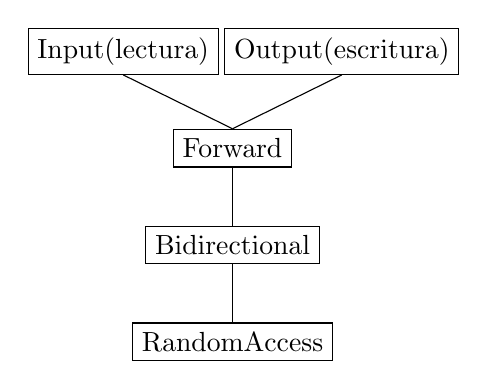
\begin{tikzpicture}[every tree node/.style=draw,grow=up]
            \tikzset{level distance=35pt}
            \Tree [.{RandomAccess}
                     [.{Bidirectional}
                        [.{Forward}
                           [.{Output(escritura)} ]
                           [.{Input(lectura)} ]
                        ]
                     ]
                  ]
            \end{tikzpicture}
\end{center}
\end{frame}
\note[itemize] {
\item Existe una jerarqu\'ia de iteradores. Todos los iteradores con RandomAccess son iteradores Bidirectionales pero no todos los Bidirectionales tienen RandomAccess
}


\begin{frame}[fragile]{Lifetime de los iteradores}{Los iteradores son v\'alidos mientras no se modifique el container}
Mal, si el container es modificado los iteradores son inv\'alidos:
   \begin{lstlisting}[style=normal]
std::list<int>::iterator it = lista.begin();
for (; it != lista.end(); ++it)
   if (*it % 2 == 0)  // remover si es par
      lista.erase(it); // el container fue modificado!!
   \end{lstlisting}
\pause
Bien:
   \begin{lstlisting}[style=normal]
std::list<int> tmp;
std::list<int>::iterator it = lista.begin();
for (; it != lista.end(); ++it) 
   if (*it % 2 != 0) // copiar si no es par
      tmp.push_back(*it);
lista.swap(tmp);
   \end{lstlisting}
\pause
Mucho mejor!:
   \begin{lstlisting}[style=normal]
bool es_par(const int &i) { return i % 2 == 0; }
std::remove_if(lista.begin(), lista.end(), es_par);
   \end{lstlisting}
\end{frame}
\note[itemize] {
\item En general un iterador es v\'alido mientras que su container no cambie: iterar un container para removerle algunos elementos suele ser un bug cl\'asico.
}

\subsection{Algoritmos}
\begin{frame}[fragile]{Algortimos gen\'ericos - Abstracci\'on de c\'odigo}
      \begin{lstlisting}[style=normal]
// no compila por un mini detalle (typename)
template <class Container, class Val>
Container::iterator find(
                        Container &v, 
                        const Val &val) {
  Container::iterator it = v.begin();
  Container::iterator end = v.end();

  while (it != end and val != *it) {
      ++it;
  }

  return it;
}
      \end{lstlisting}
\end{frame}
\begin{frame}[fragile]{Intermezzo: typenames}{Para diferenciar entre un m\'etodo y un subtipo de clase}
      \begin{lstlisting}[style=normal]
struct List {
    struct iterator {
        /* ... */
    };

    List::iterator begin() {
        return List::iterator(/*...*/);
    }
};
      \end{lstlisting}
      \begin{itemize} 
          \item \lstinline[style=normal]!List::iterator! hace referencia a un tipo (el \lstinline[style=normal]!struct iterator! dentro de \lstinline[style=normal]!List!)
          \item \lstinline[style=normal]!List::begin! hace referencia a un m\'etodo de \lstinline[style=normal]!List!
      \end{itemize}
\end{frame}


\begin{frame}[fragile]{Intermezzo: typenames}{Para diferenciar entre un m\'etodo y un subtipo de clase}
C\'omo sabe el compilador que \lstinline[style=normal]!Container::iterator! es un tipo y no un m\'etodo si ni siquiera sabe que es \lstinline[style=normal]!Container!?
      \begin{lstlisting}[style=normal]
template <class Container, class Val>
Container::iterator find(...) { ... }
      \end{lstlisting}
\pause
La keyword \lstinline[style=normal]!typename! permite diferenciar un m\'etodo de un tipo.
      \begin{lstlisting}[style=normal]
template <class Container, class Val>
typename Container::iterator find(...) { ... }
      \end{lstlisting}
\end{frame}


\begin{frame}[fragile]{Algortimos gen\'ericos - Abstracci\'on de c\'odigo}
      \begin{lstlisting}[style=normal]
// ahora si compila (siempre que Container y Val cumplan)
template <class Container, class Val>
typename Container::iterator find(
                                Container &v, 
                                const Val &val) {
  typename Container::iterator it = v.begin();
  typename Container::iterator end = v.end();

  while (it != end and val != *it) {
      ++it;
  }

  return it;
}
      \end{lstlisting}
\end{frame}

\begin{frame}[fragile]{Algoritmos con iteradores, no con containers}
      \begin{lstlisting}[style=normal]
template <class Iterator, class Val>
Iterator find(Iterator &it, Iterator &end, const Val &val) {
    while (it != end and val != *it) {
        ++it;
    }

    return it;
}
      \end{lstlisting}
\end{frame}
\note[itemize] {
\item La mayor\'ia de los algoritmos deber\'ian escribirse en t\'erminos de iteradores: recibir y retornar iteradores, independizandose del container en cuesti\'on.
}


\begin{frame}[fragile]{Algortimos de la STL: menos c\'odigo, menos bugs!}
For each, (tambi\'en conocido como map)
      \begin{lstlisting}[style=normal]
std::for_each(container.begin(), container.end(), func);
      \end{lstlisting}
\end{frame}

\begin{frame}[fragile]{Algortimos de la STL: menos c\'odigo, menos bugs!}
Como imprimir al \lstinline[style=normal]!stdout! un container (\'util para debug)
      \begin{lstlisting}[style=normal]
template<class T>
void print_to_cout(const T &val) {
    std::cout << val << " ";
}

std::list<int> l;
for_each(l.begin(), l.end(), print_to_cout<int>);
      \end{lstlisting}
\end{frame}

\begin{frame}[fragile]{Algortimos de la STL: menos c\'odigo, menos bugs!}
O con functors:
      \begin{lstlisting}[style=normal]
template<class T>
struct Printer {
    std::ostream &out;

    Printer(std::ostream &out) : out(out) {}

    void operator()(const T &val) {
        out << val << " ";
    }
};

std::list<int> l;
for_each(l.begin(), l.end(), Printer<int>(std::cout));
      \end{lstlisting}
\end{frame}

\begin{frame}[fragile]{Algortimos de la STL: menos c\'odigo, menos bugs!}
Sorting
      \begin{lstlisting}[style=normal]
// usando el operador less < como ordenador
std::sort(container.begin(), container.end());

// usando la funcion/functor especifica
std::sort(container.begin(), container.end(), less_func); 

// orden estable
std::stable_sort(container.begin(), container.end());
      \end{lstlisting}
\vphantom{X}
Searching (sobre containers ordenados)
      \begin{lstlisting}[style=normal]
// usando la misma funcion/functor que se uso para el
// ordenamiento (el operador less < es el default)
std::binary_seach(container.begin(), container.end(), 
                  val_to_be_found); 
      \end{lstlisting}
\end{frame}



\begin{frame}[fragile]{Algortimos de la STL: c\'odigo con optimizaciones}
Swap, con implementaciones especializadas para containers
      \begin{lstlisting}[style=normal]
int a = 1, b = 2;
std::swap(a, b);     // a == 2, b == 1 haciendo copias

std::list<int> a;
std::list<int> b;
std::swap(a, b);     // solo swap de punteros internos!
      \end{lstlisting}
\end{frame}



\begin{frame}[fragile]{STL - Resumen}
   \begin{itemize}
      \item El uso de templates, containers e iteradores puede dejar el c\'odigo muy verbose, usar \lstinline[style=normal]!typedef! y \lstinline[style=normal]!using!
      \item Usar el operador de preincremento \lstinline[style=normal]!++it! y no el de pos incremento para evitar copias.
      \item Busquen! \lstinline[style=normal]!std::stack!, \lstinline[style=normal]!std::queue!, \lstinline[style=normal]!std::make_heap!, \lstinline[style=normal]!std::set_intersection!, \lstinline[style=normal]!std::set_union!, etc. Hay m\'as contenedores y algoritmos listos para ser usados. \alert{Encuentrenlos y usenlos!}
   \end{itemize}
\end{frame}


\appendix
\section<presentation>*{\appendixname}
\subsection<presentation>*{Referencias}

\begin{frame}[allowframebreaks]
   \frametitle<presentation>{Referencias}

   \begin{thebibliography}{10}

         \beamertemplatebookbibitems
         % Start with overview books.
      \bibitem{cplusplus}
         http://cplusplus.com

      \bibitem{Sutter}
         Herb Sutter.
         \newblock {\em Exceptional C++: 47 Engineering Puzzles}.
         \newblock Addison Wesley, 1999.

      \bibitem{Stroustrup}
         Bjarne Stroustrup.
         \newblock {\em The C++ Programming Language}.
         \newblock Addison Wesley, Fourth Edition.

         %\beamertemplatearticlebibitems
         % Followed by interesting articles. Keep the list short. 

   \end{thebibliography}
\end{frame}

\end{document}


